\documentclass{ximera}

%\usepackage{todonotes}

\newcommand{\todo}{}

\usepackage{esint} % for \oiint
\ifxake%%https://math.meta.stackexchange.com/questions/9973/how-do-you-render-a-closed-surface-double-integral
\renewcommand{\oiint}{{\large\bigcirc}\kern-1.56em\iint}
\fi


\graphicspath{
  {./}
  {ximeraTutorial/}
  {basicPhilosophy/}
  {functionsOfSeveralVariables/}
  {normalVectors/}
  {lagrangeMultipliers/}
  {vectorFields/}
  {greensTheorem/}
  {shapeOfThingsToCome/}
  {dotProducts/}
  {partialDerivativesAndTheGradientVector/}
  {../productAndQuotientRules/exercises/}
  {../normalVectors/exercisesParametricPlots/}
  {../continuityOfFunctionsOfSeveralVariables/exercises/}
  {../partialDerivativesAndTheGradientVector/exercises/}
  {../directionalDerivativeAndChainRule/exercises/}
  {../commonCoordinates/exercisesCylindricalCoordinates/}
  {../commonCoordinates/exercisesSphericalCoordinates/}
  {../greensTheorem/exercisesCurlAndLineIntegrals/}
  {../greensTheorem/exercisesDivergenceAndLineIntegrals/}
  {../shapeOfThingsToCome/exercisesDivergenceTheorem/}
  {../greensTheorem/}
  {../shapeOfThingsToCome/}
  {../separableDifferentialEquations/exercises/}
  {vectorFields/}
}

\newcommand{\mooculus}{\textsf{\textbf{MOOC}\textnormal{\textsf{ULUS}}}}

\usepackage{tkz-euclide}
\usepackage{tikz}
\usepackage{tikz-cd}
\usetikzlibrary{arrows}
\tikzset{>=stealth,commutative diagrams/.cd,
  arrow style=tikz,diagrams={>=stealth}} %% cool arrow head
\tikzset{shorten <>/.style={ shorten >=#1, shorten <=#1 } } %% allows shorter vectors

\usetikzlibrary{backgrounds} %% for boxes around graphs
\usetikzlibrary{shapes,positioning}  %% Clouds and stars
\usetikzlibrary{matrix} %% for matrix
\usepgfplotslibrary{polar} %% for polar plots
\usepgfplotslibrary{fillbetween} %% to shade area between curves in TikZ
%\usetkzobj{all}
\usepackage[makeroom]{cancel} %% for strike outs
%\usepackage{mathtools} %% for pretty underbrace % Breaks Ximera
%\usepackage{multicol}
\usepackage{pgffor} %% required for integral for loops



%% http://tex.stackexchange.com/questions/66490/drawing-a-tikz-arc-specifying-the-center
%% Draws beach ball
\tikzset{pics/carc/.style args={#1:#2:#3}{code={\draw[pic actions] (#1:#3) arc(#1:#2:#3);}}}



\usepackage{array}
\setlength{\extrarowheight}{+.1cm}
\newdimen\digitwidth
\settowidth\digitwidth{9}
\def\divrule#1#2{
\noalign{\moveright#1\digitwidth
\vbox{\hrule width#2\digitwidth}}}




% \newcommand{\RR}{\mathbb R}
% \newcommand{\R}{\mathbb R}
% \newcommand{\N}{\mathbb N}
% \newcommand{\Z}{\mathbb Z}

\newcommand{\sagemath}{\textsf{SageMath}}


%\renewcommand{\d}{\,d\!}
%\renewcommand{\d}{\mathop{}\!d}
%\newcommand{\dd}[2][]{\frac{\d #1}{\d #2}}
%\newcommand{\pp}[2][]{\frac{\partial #1}{\partial #2}}
% \renewcommand{\l}{\ell}
%\newcommand{\ddx}{\frac{d}{\d x}}

% \newcommand{\zeroOverZero}{\ensuremath{\boldsymbol{\tfrac{0}{0}}}}
%\newcommand{\inftyOverInfty}{\ensuremath{\boldsymbol{\tfrac{\infty}{\infty}}}}
%\newcommand{\zeroOverInfty}{\ensuremath{\boldsymbol{\tfrac{0}{\infty}}}}
%\newcommand{\zeroTimesInfty}{\ensuremath{\small\boldsymbol{0\cdot \infty}}}
%\newcommand{\inftyMinusInfty}{\ensuremath{\small\boldsymbol{\infty - \infty}}}
%\newcommand{\oneToInfty}{\ensuremath{\boldsymbol{1^\infty}}}
%\newcommand{\zeroToZero}{\ensuremath{\boldsymbol{0^0}}}
%\newcommand{\inftyToZero}{\ensuremath{\boldsymbol{\infty^0}}}



% \newcommand{\numOverZero}{\ensuremath{\boldsymbol{\tfrac{\#}{0}}}}
% \newcommand{\dfn}{\textbf}
% \newcommand{\unit}{\,\mathrm}
% \newcommand{\unit}{\mathop{}\!\mathrm}
% \newcommand{\eval}[1]{\bigg[ #1 \bigg]}
% \newcommand{\seq}[1]{\left( #1 \right)}
% \renewcommand{\epsilon}{\varepsilon}
% \renewcommand{\phi}{\varphi}


% \renewcommand{\iff}{\Leftrightarrow}

% \DeclareMathOperator{\arccot}{arccot}
% \DeclareMathOperator{\arcsec}{arcsec}
% \DeclareMathOperator{\arccsc}{arccsc}
% \DeclareMathOperator{\si}{Si}
% \DeclareMathOperator{\scal}{scal}
% \DeclareMathOperator{\sign}{sign}


%% \newcommand{\tightoverset}[2]{% for arrow vec
%%   \mathop{#2}\limits^{\vbox to -.5ex{\kern-0.75ex\hbox{$#1$}\vss}}}
% \newcommand{\arrowvec}[1]{{\overset{\rightharpoonup}{#1}}}
% \renewcommand{\vec}[1]{\arrowvec{\mathbf{#1}}}
% \renewcommand{\vec}[1]{{\overset{\boldsymbol{\rightharpoonup}}{\mathbf{#1}}}}

% \newcommand{\point}[1]{\left(#1\right)} %this allows \vector{ to be changed to \vector{ with a quick find and replace
% \newcommand{\pt}[1]{\mathbf{#1}} %this allows \vec{ to be changed to \vec{ with a quick find and replace
% \newcommand{\Lim}[2]{\lim_{\point{#1} \to \point{#2}}} %Bart, I changed this to point since I want to use it.  It runs through both of the exercise and exerciseE files in limits section, which is why it was in each document to start with.

% \DeclareMathOperator{\proj}{\mathbf{proj}}
% \newcommand{\veci}{{\boldsymbol{\hat{\imath}}}}
% \newcommand{\vecj}{{\boldsymbol{\hat{\jmath}}}}
% \newcommand{\veck}{{\boldsymbol{\hat{k}}}}
% \newcommand{\vecl}{\vec{\boldsymbol{\l}}}
% \newcommand{\uvec}[1]{\mathbf{\hat{#1}}}
% \newcommand{\utan}{\mathbf{\hat{t}}}
% \newcommand{\unormal}{\mathbf{\hat{n}}}
% \newcommand{\ubinormal}{\mathbf{\hat{b}}}

% \newcommand{\dotp}{\bullet}
% \newcommand{\cross}{\boldsymbol\times}
% \newcommand{\grad}{\boldsymbol\nabla}
% \newcommand{\divergence}{\grad\dotp}
% \newcommand{\curl}{\grad\cross}
%\DeclareMathOperator{\divergence}{divergence}
%\DeclareMathOperator{\curl}[1]{\grad\cross #1}
% \newcommand{\lto}{\mathop{\longrightarrow\,}\limits}

% \renewcommand{\bar}{\overline}

\colorlet{textColor}{black}
\colorlet{background}{white}
\colorlet{penColor}{blue!50!black} % Color of a curve in a plot
\colorlet{penColor2}{red!50!black}% Color of a curve in a plot
\colorlet{penColor3}{red!50!blue} % Color of a curve in a plot
\colorlet{penColor4}{green!50!black} % Color of a curve in a plot
\colorlet{penColor5}{orange!80!black} % Color of a curve in a plot
\colorlet{penColor6}{yellow!70!black} % Color of a curve in a plot
\colorlet{fill1}{penColor!20} % Color of fill in a plot
\colorlet{fill2}{penColor2!20} % Color of fill in a plot
\colorlet{fillp}{fill1} % Color of positive area
\colorlet{filln}{penColor2!20} % Color of negative area
\colorlet{fill3}{penColor3!20} % Fill
\colorlet{fill4}{penColor4!20} % Fill
\colorlet{fill5}{penColor5!20} % Fill
\colorlet{gridColor}{gray!50} % Color of grid in a plot

\newcommand{\surfaceColor}{violet}
\newcommand{\surfaceColorTwo}{redyellow}
\newcommand{\sliceColor}{greenyellow}




\pgfmathdeclarefunction{gauss}{2}{% gives gaussian
  \pgfmathparse{1/(#2*sqrt(2*pi))*exp(-((x-#1)^2)/(2*#2^2))}%
}


%%%%%%%%%%%%%
%% Vectors
%%%%%%%%%%%%%

%% Simple horiz vectors
\renewcommand{\vector}[1]{\left\langle #1\right\rangle}


%% %% Complex Horiz Vectors with angle brackets
%% \makeatletter
%% \renewcommand{\vector}[2][ , ]{\left\langle%
%%   \def\nextitem{\def\nextitem{#1}}%
%%   \@for \el:=#2\do{\nextitem\el}\right\rangle%
%% }
%% \makeatother

%% %% Vertical Vectors
%% \def\vector#1{\begin{bmatrix}\vecListA#1,,\end{bmatrix}}
%% \def\vecListA#1,{\if,#1,\else #1\cr \expandafter \vecListA \fi}

%%%%%%%%%%%%%
%% End of vectors
%%%%%%%%%%%%%

%\newcommand{\fullwidth}{}
%\newcommand{\normalwidth}{}



%% makes a snazzy t-chart for evaluating functions
%\newenvironment{tchart}{\rowcolors{2}{}{background!90!textColor}\array}{\endarray}

%%This is to help with formatting on future title pages.
\newenvironment{sectionOutcomes}{}{}



%% Flowchart stuff
%\tikzstyle{startstop} = [rectangle, rounded corners, minimum width=3cm, minimum height=1cm,text centered, draw=black]
%\tikzstyle{question} = [rectangle, minimum width=3cm, minimum height=1cm, text centered, draw=black]
%\tikzstyle{decision} = [trapezium, trapezium left angle=70, trapezium right angle=110, minimum width=3cm, minimum height=1cm, text centered, draw=black]
%\tikzstyle{question} = [rectangle, rounded corners, minimum width=3cm, minimum height=1cm,text centered, draw=black]
%\tikzstyle{process} = [rectangle, minimum width=3cm, minimum height=1cm, text centered, draw=black]
%\tikzstyle{decision} = [trapezium, trapezium left angle=70, trapezium right angle=110, minimum width=3cm, minimum height=1cm, text centered, draw=black]


\title{Indeterminate}

\begin{document}

\begin{abstract}
no dominance
\end{abstract}
\maketitle





Functions can dominate other functions, or they can approach infinity similarly.  If the two functions approach infinity similarly, then the limit of their quotient equals a number.  The graph of the quotient approaches a horizontal asymptote. \\

This goes for $0$ as well. \\






\begin{example}

Consider the function $B(t) = \frac{3e^t - 5}{e^t + 1}$. \\

As $t \to \infty$, the exponential pieces will dominate the constant pieces.  

\[   B(t) = \frac{3e^t - 5}{e^t + 1} \sim \frac{3 e^t}{e^t} = 3   \]




As $t \to -\infty$, we have a different story.  $\lim\limits_{t \to -\infty} e^t = 0$. Therefore, in this case, the constant terms dominate.


\[   B(t) = \frac{3e^t - 5}{e^t + 1} \sim \frac{-5}{1} = -5   \]


The graph has two different horizontal asymptotes.






\begin{image}
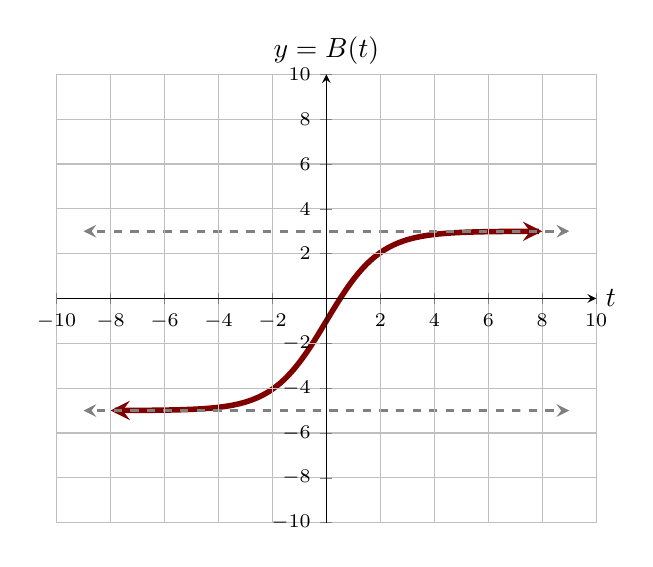
\begin{tikzpicture}
  \begin{axis}[
            domain=-10:10, ymax=10, xmax=10, ymin=-10, xmin=-10,
            axis lines =center, xlabel=$t$, ylabel={$y=B(t)$}, grid = major,
            ytick={-10,-8,-6,-4,-2,2,4,6,8,10},
            xtick={-10,-8,-6,-4,-2,2,4,6,8,10},
            yticklabels={$-10$,$-8$,$-6$,$-4$,$-2$,$2$,$4$,$6$,$8$,$10$}, 
            xticklabels={$-10$,$-8$,$-6$,$-4$,$-2$,$2$,$4$,$6$,$8$,$10$},
            ticklabel style={font=\scriptsize},
            every axis y label/.style={at=(current axis.above origin),anchor=south},
            every axis x label/.style={at=(current axis.right of origin),anchor=west},
            axis on top
          ]

            \addplot [line width=2, penColor2, smooth,samples=100,domain=(-8:8),<->] {(3*(e^x) - 5)/(e^x + 1))};
 
            \addplot [line width=1, gray, dashed,samples=200,domain=(-9:9),<->] {3};
            \addplot [line width=1, gray, dashed,samples=200,domain=(-9:9),<->] {-5};

  \end{axis}
\end{tikzpicture}
\end{image}






\end{example}








\section*{Indeterminate Forms}


We have been examining functions that approach infinity (or $0$) similarly. When combine similar functions into a new quotient function, this new function might have a contant end-behavior. \\

The problem is that a fraction of the form $\frac{very \, big}{very \, big}$ could equal anything.



\[  \frac{10000000000}{2000000000} = 50      \]

\[  \frac{1000000000}{2000000000} = \frac{1}{2}      \]

\[  \frac{1000000000}{20000000000} = 0.2      \]





The same thing happens with values near $0$


\[  \frac{0.000000001}{0.0000000002} = 50      \]

\[  \frac{0.000000001}{0.000000002} = \frac{1}{2}      \]

\[  \frac{0.0000000001}{0.0000000002} = 0.2      \]





Formulas whose values seem like they are approaching $\frac{\infty}{\infty}$ or $\frac{0}{0}$ are called \textbf{indeterminate forms}, because you can't easily determine their values.





\begin{example}  Indeterminate Forms

Both the functions $S(t) = \sqrt{2t^3 - 5}$ and $L(t) = t\sqrt{9t+4}$ approach $\infty$ as $t \to \infty$. \\



$R(t) = \frac{S(t)}{L(t)} = \frac{\sqrt{2t^3 - 5}}{t\sqrt{9t+4}}$ is an indeterminate form. It is approaching the form $\frac{\infty}{\infty}$ \\




\[
\frac{S(t)}{L(t)} = \frac{\sqrt{2t^3 - 5}}{t\sqrt{9t+4}} \sim \frac{\infty}{\infty}
\]





If we examine the quotient in terms of dominance, then we think like...

\[
R(t) =  \frac{\sqrt{2t^3 - 5}}{t \sqrt{9t+4}} \sim \frac{\sqrt{2t^3}}{t \sqrt{9t}} = \frac{t \sqrt{2t}}{t \sqrt{9t}} = \frac{\sqrt{2}}{\sqrt{9}}
\]



\[
\lim\limits_{t \to \infty} R(t) = \frac{\sqrt{2}}{3}
\]

\end{example}




When we encounter a formula that behaves like $\frac{\infty}{\infty}$, then we know we are looking at the wrong formula.   Calculations that start looking like $\frac{\infty}{\infty}$ tell us to find a different equivalent formula. \\



























\section*{Calculus}


We are introducing the term \textbf{indeterminate form} here in connection to dominance and horizontal asymptotes.  In Calculus, this idea will be expanded significantly to include other targets besides $\infty$.




\begin{example} Indeterminate Forms

Both the functions $S(t) = \sin(t)$ and $L(t) = t$ approach $0$ as $t \to 0$. \\

Do they approach $0$ similarly? \\

Let's investigate $R(t) = \frac{\sin(t)}{t}$










\begin{image}
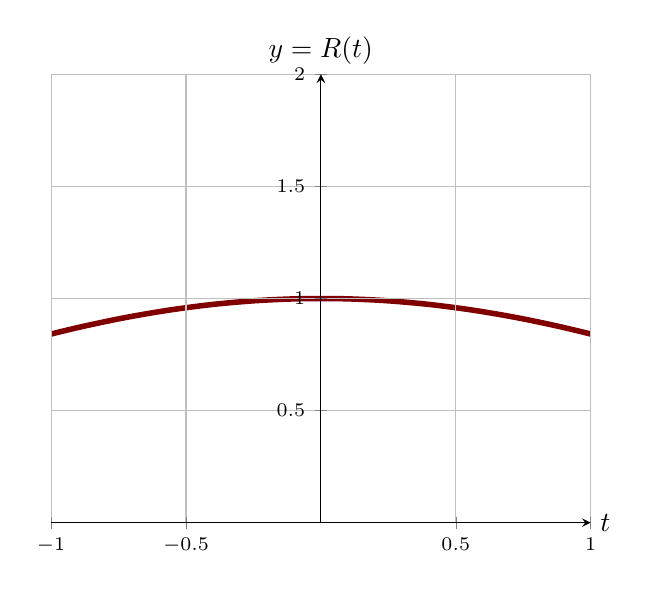
\begin{tikzpicture}
  \begin{axis}[
            domain=-1:1, ymax=2, xmax=1, ymin=0, xmin=-1,
            axis lines =center, xlabel=$t$, ylabel={$y=R(t)$}, grid = major,
            %ytick={-10,-8,-6,-4,-2,2,4,6,8,10},
            %xtick={-10,-8,-6,-4,-2,2,4,6,8,10},
            %yticklabels={$-10$,$-8$,$-6$,$-4$,$-2$,$2$,$4$,$6$,$8$,$10$}, 
            %xticklabels={$-10$,$-8$,$-6$,$-4$,$-2$,$2$,$4$,$6$,$8$,$10$},
            ticklabel style={font=\scriptsize},
            every axis y label/.style={at=(current axis.above origin),anchor=south},
            every axis x label/.style={at=(current axis.right of origin),anchor=west},
            axis on top
          ]
          

            \addplot [line width=2, penColor2, smooth,samples=100,domain=(-8:8),<->] {sin(deg(x))/x};





           

  \end{axis}
\end{tikzpicture}
\end{image}







The graph is very suggestive that $\sin(t)$ and $t$ approach $0$ in exactly the same way.  Their quotient approaches $1$.



\end{example}
















\begin{example} Indeterminate Forms

We have seen an even weirder indeterminate form.

Everyone knows that $1$ to any power equals $1$. Everyone knows that numbers greater than $1$ to bigger powers get bigger.


What about something like $\left( 1 + \frac{1}{x} \right)^x$ ?

The base is getting closer to $1$, but it is always greater than $1$.  The power is growing larger.  

We are heading to something like $1^{\infty}$.

And we have seen this function actually approaches the value $e \approx 2.71828$. \\

How far out in the domain do you need to go for the graph to be inside the interval $[2.7, 2.8]$?








\begin{center}
\desmos{ttk7altjct}{400}{300}
\end{center}









\end{example}



Calculus will investigate the ideas of indeterminance in detail.  We are just getting started.










\begin{center}
\textbf{\textcolor{green!50!black}{ooooo-=-=-=-ooOoo-=-=-=-ooooo}} \\

more examples can be found by following this link\\ \link[More Examples of Dominance]{https://ximera.osu.edu/csccmathematics/precalculus1/precalculus1/functionComparison/examples/exampleList}

\end{center}





\end{document}
